\documentclass[11pt]{article}

\usepackage[utf8]{inputenc}
\usepackage[T1]{fontenc}
\usepackage{times}
\usepackage{booktabs}
\usepackage{url}
\usepackage{graphicx}
\usepackage{tikz}
\usetikzlibrary{arrows.meta,positioning}
\usepackage[numbers,sort&compress]{natbib}
\usepackage[hidelinks]{hyperref}
\usepackage{xcolor}

\newcommand{\aifeed}{AIFeed}
\newcommand{\aimd}{AIFeed Markdown}
\newcommand{\mako}{MAKO}
\newcommand{\code}[1]{\texttt{#1}}

\title{\aifeed{}: Verifiable Content Permissions and\\
Efficient Agent Delivery for the AI Web}
\author{AIFeed Protocol Contributors\thanks{Contact: \texttt{contact@aifeed.md}
(submission contact; to be confirmed). Artifacts:
\url{https://github.com/denyn1/aifeed-protocol}.}}
\date{Draft --- \today}

\begin{document}
\maketitle

\begin{abstract}
AI systems now consume more web content than people do, and the plain-text preferences in
\code{robots.txt} do not hold them back: one vendor logged 1.9 billion crawls that ignored
robots rules in a single half-year, and one web-only measurement put the crawl-to-referral
ratio of a major AI provider at 70{,}900:1. Preference and licensing signals exist, but
they are not attributable to a domain, cannot be revoked, and do nothing about the cost of
repeated consumption. We describe \aifeed{}, an open trust layer built around a signed
manifest of machine-readable permissions, anchored in DNS and checked against a
multi-signature revocation registry. Two content profiles ride on the same signed bytes: a
native markdown format (\aimd{}) and a compatibility profile for the external \mako{}
draft. Three properties, taken together, distinguish the design from the signals we
surveyed: signed provenance of permissions, per-page binding with restrict-only overrides,
and a digest-bearing delta index that lets an agent skip pages that have not changed.
We measure the system on committed artifacts. Converting a 60-page corpus to the markdown
profiles cuts transferred bytes by 68.8\% (95.7\% for delta consumption), and a loopback
enforcement harness with four client profiles records publisher savings of 55.2\% of bytes
and 56.2\% of CPU, AI-side savings of 54.8\% (72.9\% for the compliant client), 14 of 18
unchanged pages skipped, and signature verification at 0.70\,ms per page. The
specification is exercised by 34 manifest, 39 \mako{}, and 11 \aimd{} vectors under
independent JavaScript and Python verifiers, plus differential PHP fixtures and an
end-to-end WordPress deployment. We also report results that do not flatter the design:
without adoption and enforcement there are no savings at all; vendor claims of up to 94\%
token reduction rely on summarization our converter does not perform; origin-plus-DNS
compromise is invisible on first contact; and the compatibility profile depends on a
third-party draft. No external cryptographic review or live pilot exists yet.
\end{abstract}

\section{Introduction}

Web content is increasingly consumed by automated agents rather than human visitors.
Cloudflare's radar puts AI bots at an average of 4.2\% of HTML requests in 2025 (6.4\% at
peak), with automated traffic approaching half of all HTML requests and ``user action''
agent crawls growing more than 15-fold over the same period~\citep{cfRadar2025}. The
publisher-facing asymmetry is worse than those aggregates suggest: one web-only
measurement found a crawl-to-referral ratio of 70{,}900:1 for a major AI
provider~\citep{cfCrawlRefer}, and a single vendor recorded 22 billion AI scrapes in a
half-year, 1.9 billion of which ignored \code{robots.txt}~\citep{tollbit}.

The ecosystem is not empty. RFC~9309 and the IETF AIPREF drafts cover robotic preferences;
Cloudflare's Content Signals, RSL, and the W3C TDM Reservation Protocol each express some
flavor of permission or license~\citep{rfc9309,draftAiprefVocab,draftAiprefAttach,cfContentSignals,rsl,tdmrep};
\code{llms.txt} indexes a site for language models~\citep{llmstxt}; and on the other side
of the exchange, Web Bot Auth is putting signed agent requests into
production~\citep{draftWebbotauth,cfBotPrinciples}. What is missing is twofold. A
publisher's declaration is not attributable: any intermediary can alter it, and nothing
standard lets the publisher revoke it. And even a declaration that is respected leaves the
mechanical cost untouched, because agents keep pulling unchanged pages as browser-shaped
HTML.

We make four contributions:

\begin{enumerate}
  \item \textbf{Design.} \aifeed{} v0.1: an Ed25519-signed, JCS-canonicalized manifest at
  \code{/.well-known/ai.json}, cryptographically anchored to the domain through a DNS TXT
  record, servable offline, with a multi-signature revocation registry and bounded
  staleness semantics.
  \item \textbf{Content profiles.} \aifeed{} v0.2 adds signed per-page content delivery:
  the native \aimd{} profile (\code{text/aifeed+markdown}) with first-class permission,
  asset, and triage metadata; the \mako{} compatibility profile; restrict-only per-page
  overrides; and a digest-bearing delta index with a site resume and per-entry triage
  fields.
  \item \textbf{Implementation.} A zero-dependency reference stack: CLI, JavaScript SDK,
  independent Python verifier, WordPress publisher plugin, static-site builder, and
  server adapters for nginx, Caddy, Apache, Node, Next.js, PHP, Python ASGI, and Go.
  \item \textbf{Evaluation and reproducibility.} Measured conversion, delta, and
  enforcement results with committed artifacts, conformance vectors, fuzzing, and
  differential cross-language testing; unfavorable results are reported alongside them.
\end{enumerate}

\section{Background and Related Work}

\paragraph{Preference and permission signals.}
Robots preferences were standardized in RFC~9309~\citep{rfc9309}, and the IETF AIPREF
working group is now assembling a vocabulary for AI usage preferences together with an
attachment mechanism for HTTP responses~\citep{draftAiprefVocab,draftAiprefAttach}.
Industry has moved faster: Cloudflare's Content Signals Policy expresses search, AI-input,
and AI-training preferences and reports adoption on more than 3.8M domains through managed
robots files~\citep{cfContentSignals}, with pay-per-crawl billing offered at the same
edge~\citep{cfPayPerCrawl}; RSL adds licensing and compensation
terms~\citep{rsl}; the W3C TDM Reservation Protocol handles text-and-data-mining
reservations~\citep{tdmrep}; and \code{llms.txt} gives language models a site-level
content index~\citep{llmstxt}. What none of these provides is attribution of the
declaration to the domain, a revocation path, or verification that does not depend on the
transport channel.

\paragraph{Agent-side authentication.}
Web Bot Auth defines HTTP message signatures for automated traffic, built on RFC~9421 and
Ed25519~\citep{draftWebbotauth,draftWebbotArch,rfc9421,rfc8032}. Production deployments
include a major assistant signing its agent requests and a platform verifying
them~\citep{cfBotPrinciples}. \aifeed{} uses the same primitives in the opposite
direction---the publisher signs---so the two directions compose rather than compete.

\paragraph{Content formats for agents.}
\mako{} defines a per-page markdown format with YAML frontmatter, semantic links,
declared actions, and experimental compact embeddings, and explicitly leaves authenticity
verification out of scope~\citep{makoSpec}; vendor ``markdown for agents'' conversion
exists at the CDN edge. Several projects from 2026 occupy adjacent ground.
\code{ai-policy.json} gathers permission declarations at a well-known URL, though without
signatures, anchoring, or revocation~\citep{aipolicyjson}; \code{agents.txt} puts identity,
terms, and endpoints in a root file~\citep{agentstxt}; CrawlWall enforces crawler policy at
the edge and keeps a signed audit ledger with receipts~\citep{crawlwall}; and
\code{terms.txt} goes furthest, specifying per-path, per-purpose terms with a signed
exchange, delegation tokens, and payment negotiation~\citep{chowdhury2026}. On the
academic side, \code{ai.txt} proposes a domain-specific language for guiding AI
interactions~\citep{li2025aitxt}. As of our inspection (2026-09-15), we did not find a
single project that combines publisher-signed permissions with a DNS anchor and
multi-signature revocation, a native agent format plus a compatibility profile over one
signed payload, and a digest-bearing delta index with verifiable per-page triage. Our
claim is to that combination, not to having invented any of its parts.

\paragraph{Measurement and economics.}
A substantial empirical literature studies robots at scale: classifier-based analysis of
robots usage~\citep{lee2009}, exclusion as a guidance protocol~\citep{ge2016},
robots-based gatekeeping~\citep{steinacker2025}, the efficacy of creator protection
against AI crawlers (IMC~2025)~\citep{liu2025}, bot protection for small
organizations~\citep{hoetzlein2026}, agent compliance with in-band governance
signals~\citep{munirathinam2026}, and pay-per-crawl pricing~\citep{archer2026}. Industry
reports supply the traffic asymmetry that motivates this work
\citep{cfRadar2025,tollbit,cfCrawlRefer,cfContentIndependence}, and a research center
documents how AI summaries affect users~\citep{pew2025}. On the regulatory side we note
the EU AI Act and a 2026 EU feasibility study on a TDM opt-out
registry~\citep{euAiact,euTdmRegistry}, with Indonesia's personal-data protection law as
a national example~\citep{uuPdp27}; our legal remarks are open questions, not legal
advice.

\section{Design}

\subsection{Trust chain}

\aifeed{} composes four layers, none sufficient alone: TLS (transport identity), domain
match (the manifest's \code{identity.domain} must equal the serving host), an Ed25519
signature over the JCS canonical form of the manifest with domain separation
(\code{aifeed.v0.2\textbackslash n}), and a DNS TXT anchor (\code{\_aifeed}) binding the
public key to the domain. The manifest lives at a well-known URI~\citep{rfc8615} and is
parsed under strict JSON and I-JSON rules~\citep{rfc8259,rfc7493} with RFC~3339
timestamps~\citep{rfc3339}, JCS canonicalization~\citep{rfc8785}, and BCP~14 key
words~\citep{rfc2119,rfc8174}. Figure~\ref{fig:flow} summarizes the flow. Clients persist
the first accepted key per origin to detect key replacement; the transparency log
(RFC~9162 pattern~\citep{rfc9162}) and key pinning mitigate, but do not eliminate, the
trust-on-first-use gap discussed in Section~\ref{sec:limitations}.

\begin{figure}[t]
\centering
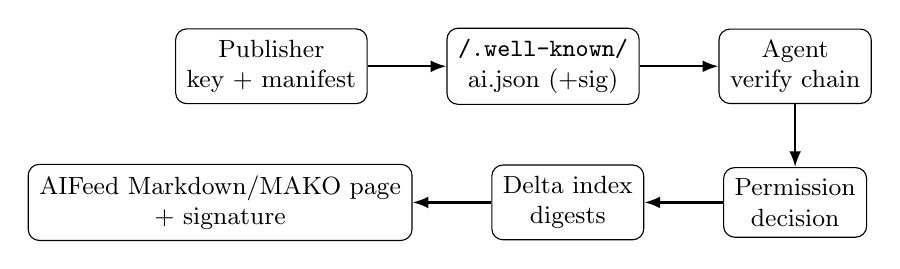
\begin{tikzpicture}[
  node distance=8mm and 10mm,
  box/.style={draw, rounded corners, align=center, font=\small, inner sep=4pt},
  arr/.style={-{Latex[length=2mm]}, thick}
]
\node[box] (pub) {Publisher\\key + manifest};
\node[box, right=of pub] (wellknown) {\code{/.well-known/}\\ai.json (+sig)};
\node[box, right=of wellknown] (agent) {Agent\\verify chain};
\node[box, below=of agent] (decide) {Permission\\decision};
\node[box, left=of decide] (index) {Delta index\\digests};
\node[box, left=of index] (page) {\aimd/\mako{} page\\+ signature};
\draw[arr] (pub) -- (wellknown);
\draw[arr] (wellknown) -- (agent);
\draw[arr] (agent) -- (decide);
\draw[arr] (decide) -- (index);
\draw[arr] (index) -- (page);
\end{tikzpicture}
\caption{High-level flow: signed manifest and DNS anchor establish attributable
permissions; the delta index selects what an agent needs; page documents carry their own
signatures bound to the page URL.}
\label{fig:flow}
\end{figure}

\subsection{Permissions and revocability}

The manifest declares a default permission and per-usage values (search, retrieval,
input, training, quote, summarize, reproduce, translate, modify, embed, commercial use),
attribution policy, and crawl limits. Revocation is served by a registry as multi-signed
documents with due-process statuses (\code{active}, \code{under\_review},
\code{suspended}) and bounded staleness: clients treat registry unavailability of more
than 168 hours as \code{UNVERIFIED}. Trust levels are explicit---\code{VERIFIED},
\code{UNVERIFIED}, \code{SUSPENDED}---and high-risk uses require a verified manifest with
a DNS anchor.

\subsection{Content profiles and per-page binding}

\aifeed{} v0.2 binds policy to individual pages. A page profile carries an \code{aifeed}
block (usage overrides, attribution, limits, license references, and asset links) that is
\emph{restrict-only} by default: a page can tighten but never loosen the origin policy.
Two profiles are supported over the same signed body bytes:

\begin{itemize}
  \item \aimd{} v1.0, the native profile~\citep{aimdSpec}: media type
  \code{text/aifeed+markdown} (media type procedures~\citep{rfc6838}, markdown media
  type~\citep{rfc7763}), extension \code{.aifeed.md}, marker \code{aimd: "1.0"},
  first-class policy block, optional translation links (\code{alternates}), and a token
  budget chosen by the publisher (reference default 4{,}000).
  \item \mako{} 1.0~\citep{makoSpec}, the compatibility profile
  (\code{text/mako+markdown}); dual-stack origins serve identical bytes under both media
  types, each with its own signature context (\code{aimd} or \code{mako}), which prevents
  cross-format replay.
\end{itemize}

A signature container binds the signed bytes to the canonical page URL
(\code{UTF-8("aifeed.aimd.v1\textbackslash n") || url || LF || raw bytes}); sidecar or
inline delivery is permitted. Converters emit referenced media and downloadable files as
links (\code{aifeed.assets}) so agents decide what to fetch, and the safe YAML subset
used for frontmatter rejects anchors, aliases, tags, flow collections, and oversized
scalars.

\subsection{Delta consumption}

The delta index (\code{/.well-known/aifeed-index.json}, signed with context
\code{aimd-index}) lists pages with \code{sha-256} digests, ETags, token counts, a site
resume, and triage fields (title, summary, tags, language, related). Clients diff digests
against stored state and fetch only changed pages; unchanged pages cost zero bytes
(conditional requests per HTTP semantics~\citep{rfc9110,rfc7231}, content digests per
RFC~9530~\citep{rfc9530}, and index discovery via web linking~\citep{rfc8288}). Index
entries are treated as untrusted claims: digests are verified against fetched bytes
before use.

\section{Threat Model}

We reuse the attack taxonomy evaluated by the conformance suite: manifests hosted on
foreign domains, content edited after signing, key replacement, origin or DNS compromise,
network modification, stale CDN copies, replays, transport corruption, and local
reformatting. The suite also covers content-profile attacks: tampered documents, digest
mismatch, cross-URL replay, cross-format/context replay, stripped signatures with
manifest policy \code{signature: required}, fail-open permission overrides, and YAML
parser abuses (anchors, aliases, tags, duplicate keys, depth/size bombs). Two properties
are explicitly \emph{not} claimed: first-contact origin+DNS compromise is undetectable
without out-of-band state; and signatures attest provenance, not the fidelity of a
markdown derivative to the HTML rendering. Enforcement is required to make declarations
effective: the 1.9 billion bypass events~\citep{tollbit} show that unenforced preferences
are advisory.

The key-replacement case is addressed by a rotation ceremony (v0.2, \S14): the successor
is announced with an old-key-signed directive plus an advisory DNS \code{pk2}
cross-check, the old key is accepted only inside a bounded overlap window, and after
cutover it is revoked permanently. This bounds, but does not eliminate, the window in
which a compromised key is still accepted, and it does not defend against an attacker
who already controls origin content and DNS.

\section{Implementation}

The reference implementation is zero-dependency~\citep{aifeedRepo}. It includes: a strict
JSON parser (duplicate keys, NFC, integer bounds) and a safe YAML-subset frontmatter
parser; JCS canonicalization and Ed25519 signing/verification; a CLI (\code{keygen},
\code{sign}, \code{validate}, \code{bundle},
\code{aimd|mako generate|sign|verify|index|fetch}, \code{site build}); an npm SDK
(\code{@aifeed/verify}) with manifest, document, index, and triage-selection APIs; an
independent Python verifier; a WordPress publisher plugin serving dual-stack content with
signed manifests, indices, assets, triage, and \code{llms.txt}; a static-site builder;
and server adapters for eight platforms. Conformance is verified by 34 manifest, 39
\mako{}, and 11 \aimd{} vectors executed by both JavaScript and Python implementations,
plus PHP differential fixtures and a WordPress end-to-end test. The specifications are
published as \aifeed{} v0.1~\citep{aifeedSpec01}, v0.2~\citep{aifeedSpec02}, and
\aimd{} v1.0~\citep{aimdSpec}.

\section{Evaluation}
\label{sec:eval}

All numbers below are reproducible from committed artifacts
(\code{benchmarks/*.json}, \code{npm run bench:mako}, \code{npm run bench:enforcement});
seeds are fixed, and the environment is a single machine with loopback networking. The
corpus is synthetic and deliberately contains navigation, ads, comments, and scripts to
model news pages.

\subsection{Content efficiency}

On a 60-page corpus, faithful conversion to the markdown profiles reduces transferred
bytes from 1{,}205{,}292 to 375{,}630 (including signature containers), a reduction of
\textbf{68.83\%}; the token estimate (bytes/4) falls by 68.8\%. Signing costs 0.25\,ms per
page; per-page verification costs 0.34--0.70\,ms. Delta consumption with 10\% of pages
changed transfers 51{,}408 bytes, \textbf{95.73\%} below the HTML crawl (the model
assumes 304 responses for unchanged pages). The \mako{} specification claims up to 94\%
token reduction; that figure presumes semantic summarization by the publisher, which our
faithful converter does not perform automatically, and we therefore report the smaller
measured conversion value rather than the vendor claim.

\subsection{Enforcement harness}

A loopback origin behind a policy-enforcement edge (training bots denied with 403;
non-compliant AI profiles rate-limited with 429 + Retry-After; humans and compliant
clients exempt) serves four deterministic client profiles across four scenarios
(Table~\ref{tab:enforce}). Scenario S3 combines training denial, rate limiting, and
delta consumption.

\begin{table}[t]
\centering
\small
\caption{Publisher-side and AI-side savings versus the no-enforcement baseline (S0);
single origin, 18-page site, real HTTP on loopback. ``bytes'' are response bodies.}
\label{tab:enforce}
\begin{tabular}{lrrrr}
\toprule
 & S0 & S1 & S2 & S3 \\
\midrule
Origin requests              & 63 & 45 & 42 & 30 \\
Origin bytes                 & 177{,}537 & 104{,}084 & 95{,}580 & 79{,}555 \\
Origin CPU (ms)              & 46.6 & 31.1 & 28.6 & 20.4 \\
Peak origin concurrency      & 17 & 4 & 2 & 2 \\
403 blocks                   & 0 & 18 & 18 & 18 \\
429 limits                   & 0 & 0 & 11 & 11 \\
Client bytes received        & 177{,}537 & 104{,}570 & 96{,}198 & 80{,}173 \\
Human p95 latency (ms)       & 20.0 & 23.2 & 19.9 & 19.3 \\
\midrule
Publisher byte saving        & -- & 41.4\% & 46.2\% & \textbf{55.2\%} \\
Publisher CPU saving         & -- & 33.4\% & 38.8\% & \textbf{56.2\%} \\
Peak-concurrency reduction   & -- & 76.5\% & 88.2\% & \textbf{88.2\%} \\
AI byte saving (all clients) & -- & 41.1\% & 45.8\% & \textbf{54.8\%} \\
AI byte saving (compliant)   & -- & 42.5\% & 42.5\% & \textbf{72.9\%} \\
\bottomrule
\end{tabular}
\end{table}

A 100-tenant run reduces origin bytes from 962{,}373 to 451{,}038 in the enforced
scenario; per-1{,}000-tenant projections are included in the artifact but are labeled as
linear extrapolations. Without enforcement (S0) savings are zero by construction, and
the bypass literature~\citep{tollbit} indicates that this baseline is realistic for
non-compliant crawlers.

\subsection{Correctness and robustness}

Across the conformance suites, signature verification failed zero times, cross-context
and cross-URL replays were rejected, and tampered documents were detected by digest
mismatch. Frontmatter and container parsers withstood 90{,}000+ fuzz executions without
invariant violations; the safe YAML subset rejects anchor, alias, tag, flow, duplicate,
and oversized inputs. The WordPress end-to-end test verifies negotiation, inline
signatures, index signatures, assets, triage fields, and \code{llms.txt} on a real
installation.

\section{Discussion}
\label{sec:limitations}

\textbf{Adoption is two-sided and enforcement-dependent.} A signed declaration has value
only if agents consume and respect it, or if an enforcement point acts on it. We
therefore position \aifeed{} as verifiable input to CDNs, WAFs, and hosting platforms
(adapter configurations are provided), not as a replacement for enforcement.

\textbf{Compatibility profile dependency.} The \mako{} profile depends on a third-party
draft specification; we pin a revision and provide a native profile (\aimd{}) so that
the protocol does not depend on a single external document. \code{terms.txt} and
\code{ai.txt} propose adjacent mechanisms; convergence or divergence will be observable
over time.

\textbf{Trust-on-first-use.} Combined origin and DNS compromise on first contact is not
cryptographically detectable; mitigations (pinning, anti-rollback, transparency log)
require client state or ecosystem participation.

\textbf{Evaluation scope.} Measurements are single-machine, loopback, and synthetic;
percentage savings depend on boilerplate ratios and on real crawler behavior. No live
30-day pilot has been completed at preprint time; a pilot kit is published so that
independent operators can reproduce and extend the measurement. Human latency effects
are bounded by the low-priority policy in our harness but not validated in production.

\textbf{Legal questions remain open.} Machine-readable reservations of rights interact
with regimes such as EU TDM opt-out requirements, whose registry feasibility is under
study~\citep{euTdmRegistry}; we flag these as legal questions requiring counsel,
consistent with the evidence labels used in the specification.

\textbf{Conflicts of interest.} The authors are the protocol's designers; mitigations are
open specifications, open conformance vectors, committed benchmark artifacts, and
reproduction commands. External cryptographic review is planned and not yet complete.

\section{Conclusion and Future Work}

\aifeed{} demonstrates that publisher-side, cryptographically attributable content
permissions can be specified, implemented without dependencies, and evaluated with
modest but reproducible gains: 55--56\% publisher-side byte and CPU savings under
enforcement, 55--73\% AI-side byte savings, and 95.7\% savings in steady-state delta
consumption, with verification costs under a millisecond per page. The remaining work is
not primarily technical: independent cryptographic review, a live pilot, upstream
standardization of the trust layer (\code{EXTENSION.md} for \mako{}; an IETF
Internet-Draft for the protocol core), and multi-stakeholder governance of the
revocation registry. We release all specifications, vectors, and harnesses so that these
claims can be challenged, reproduced, and improved.

\section*{Ethics and artifact availability}

All measurements use synthetic pages and loopback networking; no personal data is
processed. The specifications, conformance vectors, fuzzers, benchmark harnesses, and
raw results are released under MIT (code), CC BY 4.0 (specification text), and CC0
(vectors). Reproduction commands are listed in the repository README; the public
repository URL is recorded in the submission checklist.

\bibliographystyle{plainnat}
\bibliography{refs}

\end{document}
